%______________________________________________________
%
%   LaTeX-mall fr nybrjare
%
%   Konstruerad av Marcus Bergner, bergner@cs.umu.se
%
%   Vid funderingar titta lngst ned i denna fil,
%   eller skicka ett mail
%______________________________________________________
%

% lite instllningar
\documentclass[10pt, titlepage, oneside, a4paper]{article}
\usepackage[T1]{fontenc}
\usepackage[utf8]{inputenc}
\usepackage[english]{babel}
\usepackage{amssymb, graphicx, fancyheadings}
\usepackage{placeins}
\addtolength{\textheight}{20mm}
\addtolength{\voffset}{-5mm}
\renewcommand{\sectionmark}[1]{\markleft{#1}}

% \Section ger mindre spillutrymme, anvnd dem om du vill
\newcommand{\Section}[1]{\section{#1}\vspace{-8pt}}
\newcommand{\Subsection}[1]{\vspace{-4pt}\subsection{#1}\vspace{-8pt}}
\newcommand{\Subsubsection}[1]{\vspace{-4pt}\subsubsection{#1}\vspace{-8pt}}
	
% appendices, \appitem och \appsubitem r fr bilagor
\newcounter{appendixpage}

\newenvironment{appendices}{
	\setcounter{appendixpage}{\arabic{page}}
	\stepcounter{appendixpage}
}{
}

\newcommand{\appitem}[2]{
	\stepcounter{section}
	\addtocontents{toc}{\protect\contentsline{section}{\numberline{\Alph{section}}#1}{\arabic{appendixpage}}}
	\addtocounter{appendixpage}{#2}
}

\newcommand{\appsubitem}[2]{
	\stepcounter{subsection}
	\addtocontents{toc}{\protect\contentsline{subsection}{\numberline{\Alph{section}.\arabic{subsection}}#1}{\arabic{appendixpage}}}
	\addtocounter{appendixpage}{#2}
}

% ndra de rader som behver ndras
\def\inst{Department of computer science}
\def\typeofdoc{Lab report}
\def\course{Modelling and Simulation 7.5hp}
\def\pretitle{Laboratory 5}
\def\title{ODE using GSL-library}
\def\name{Robin Lundberg}
\def\username{rolu0008}
\def\email{\username{}@student.umu.se}
\def\path{/home/rolund03/workspace/gsl_ode}
\def\graders{Claude Lacoursière}


% om du vill referera till katalogen dr dina filer ligger kan du 
% anvnda \fullpath som kommer att vara "~username/edu..." o.s.v.
%\def\fullpath{\raisebox{1pt}{$\scriptstyle \sim$}\username/\path}


% Hr brjar sjlva dokumentet
\begin{document}

	% skapar framsidan (om den inte duger: gr helt enkelt en egen)
	\begin{titlepage}
		\thispagestyle{empty}
		\begin{large}
			\begin{tabular}{@{}p{\textwidth}@{}}
				\textbf{UMEÅ UNIVERSITY \hfill \today} \\
				\textbf{\inst} \\
				\textbf{\typeofdoc} \\
			\end{tabular}
		\end{large}
		\vspace{10mm}
		\begin{center}
			\LARGE{\pretitle} \\
			\huge{\textbf{\course}}\\
			\vspace{10mm}
			\LARGE{\title} \\
			\vspace{15mm}
			\begin{large}
				\begin{tabular}{ll}
					\textbf{Name} & \name \\
					\textbf{E-mail} & \texttt{\email} \\
					\textbf{Path} & \texttt{/home/rolund03/workspace/gsl\_ode} \\
				\end{tabular}
			\end{large}
			\vfill
			\large{\textbf{Supervisor}}\\
			\mbox{\large{\graders}}
		\end{center}
	\end{titlepage}


	% fixar sidfot
	\lfoot{\footnotesize{\name, \email}}
	\rfoot{\footnotesize{\today}}
	\lhead{\sc\footnotesize\title}
	\rhead{\nouppercase{\sc\footnotesize\leftmark}}
	\pagestyle{fancy}
	\renewcommand{\headrulewidth}{0.2pt}
	\renewcommand{\footrulewidth}{0.2pt}

	% skapar innehllsfrteckning.
	% Tnk p att kra latex 2ggr fr att uppdatera allt
	\pagenumbering{roman}
	\tableofcontents
	
	% och lägger in en sidbrytning
	\newpage

	\pagenumbering{arabic}

	% i Sverige har vi normalt inget indrag vid nytt stycke
	\setlength{\parindent}{0pt}
	% men dremot lite mellanrum
	\setlength{\parskip}{10pt}

	% lägger in rubrik (finns \section, men då får man mycket spillutrymme)
	\FloatBarrier
	\Section{Exercise 1}
	\begin{figure}[h!]
	\centering
	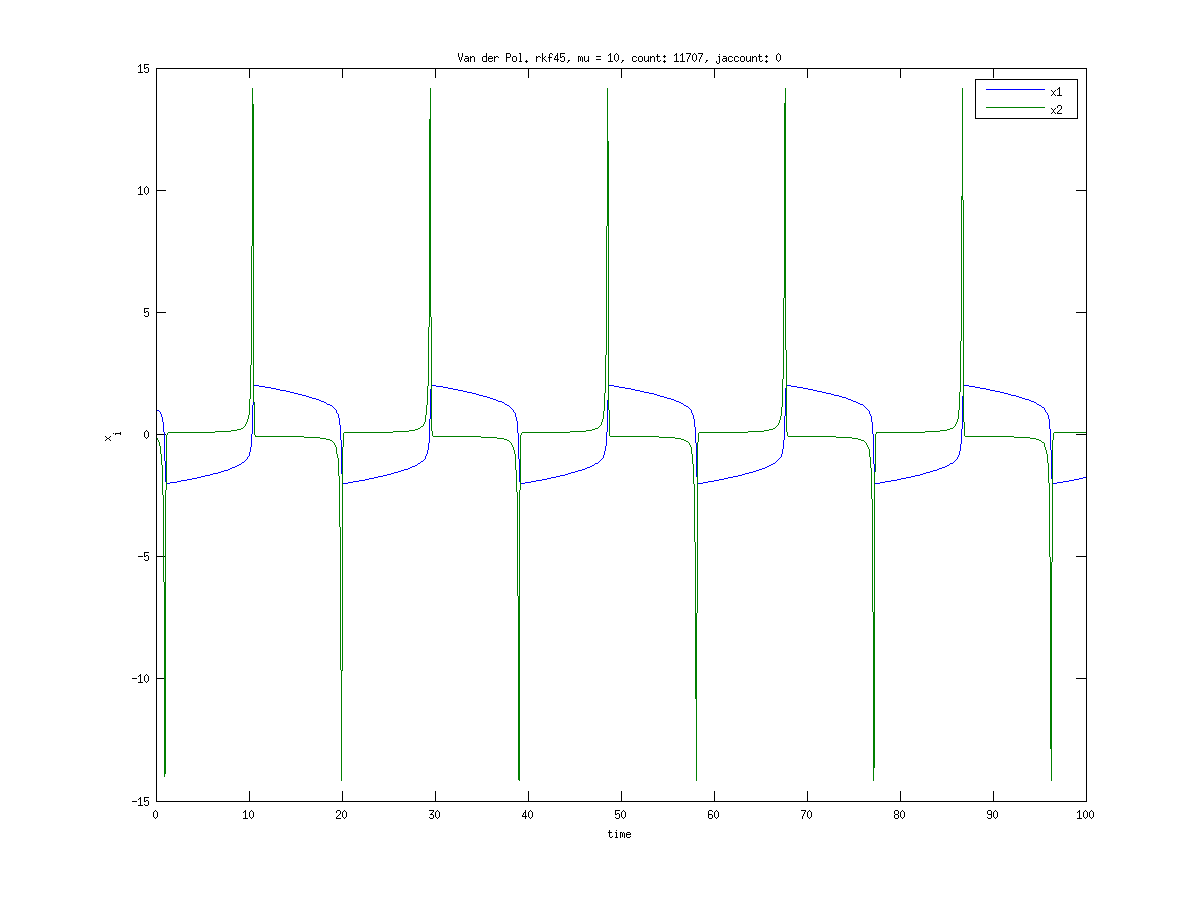
\includegraphics[width=0.8\textwidth]{img/exc1_45_10}
	\caption{Van der Pol model. Solved using rkf45 with parameter $\mu = 10$.}
	\label{fig:exc1_45_10}
\end{figure}

\begin{figure}[h!]
	\centering
	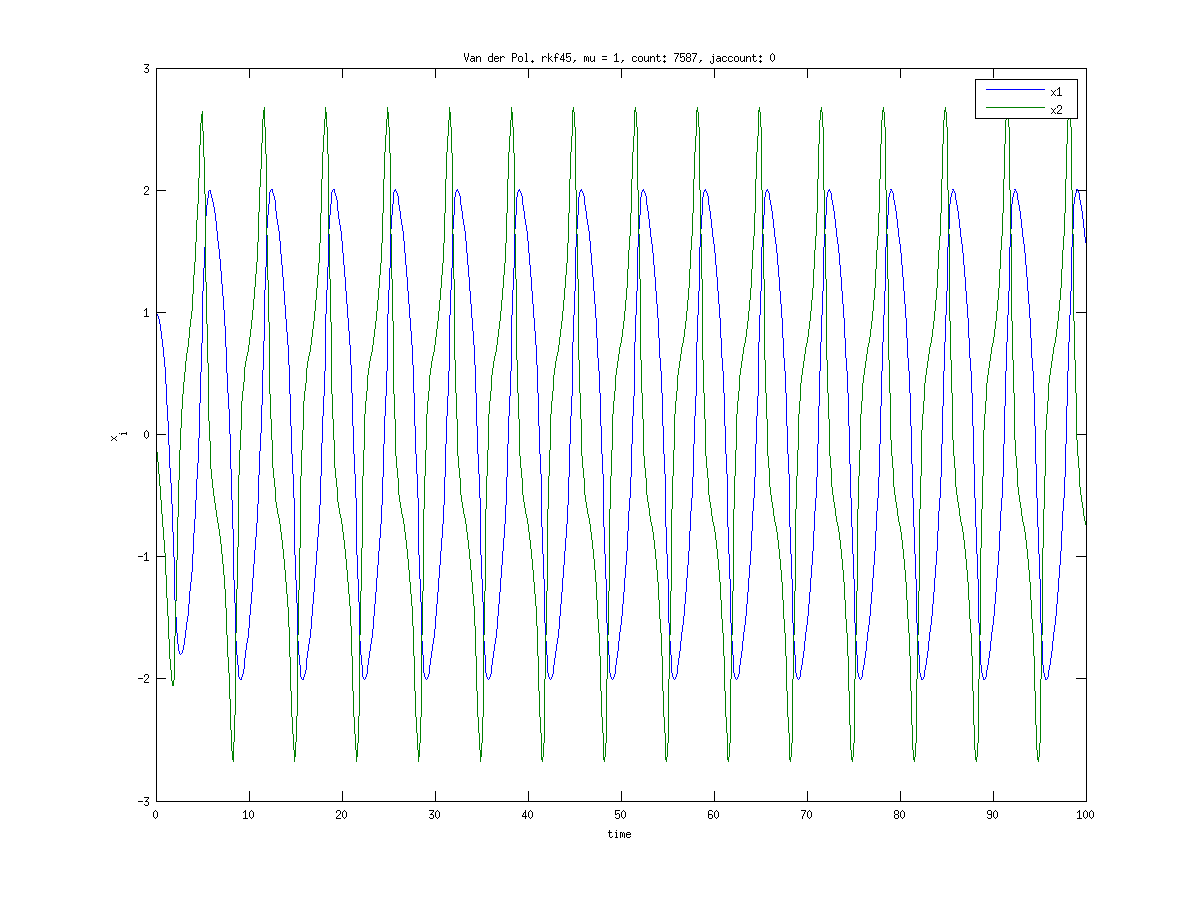
\includegraphics[width=0.8\textwidth]{img/exc1_45_1}
	\caption{Van der Pol model. Solved using rkf45 with parameter $\mu = 1$.}
	\label{fig:exc1_45_1}
\end{figure}

\begin{figure}[h!]
	\centering
	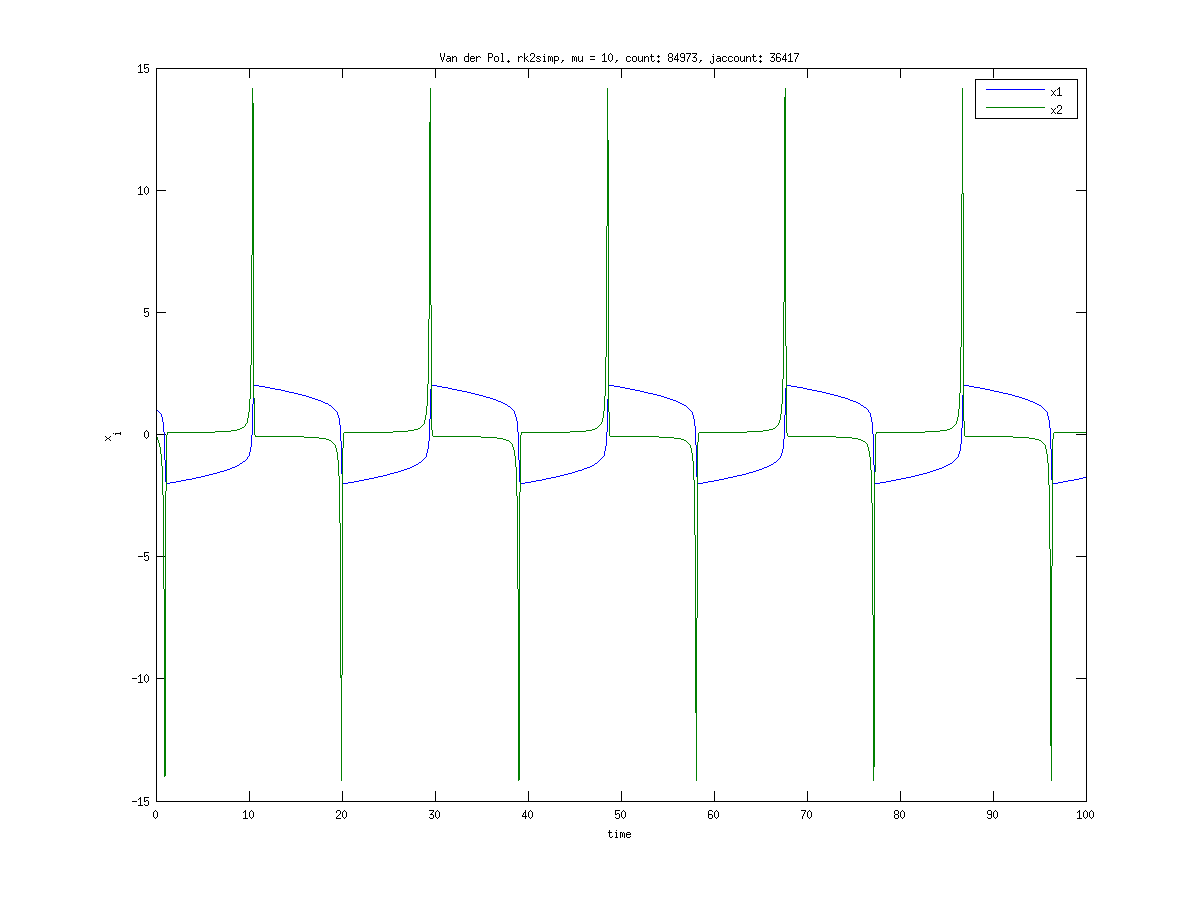
\includegraphics[width=0.8\textwidth]{img/exc1_2_10}
	\caption{Van der Pol model. Solved using rk2simp with parameter $\mu = 10$.}
	\label{fig:exc1_2_10}
\end{figure}

\begin{figure}[h!]
	\centering
	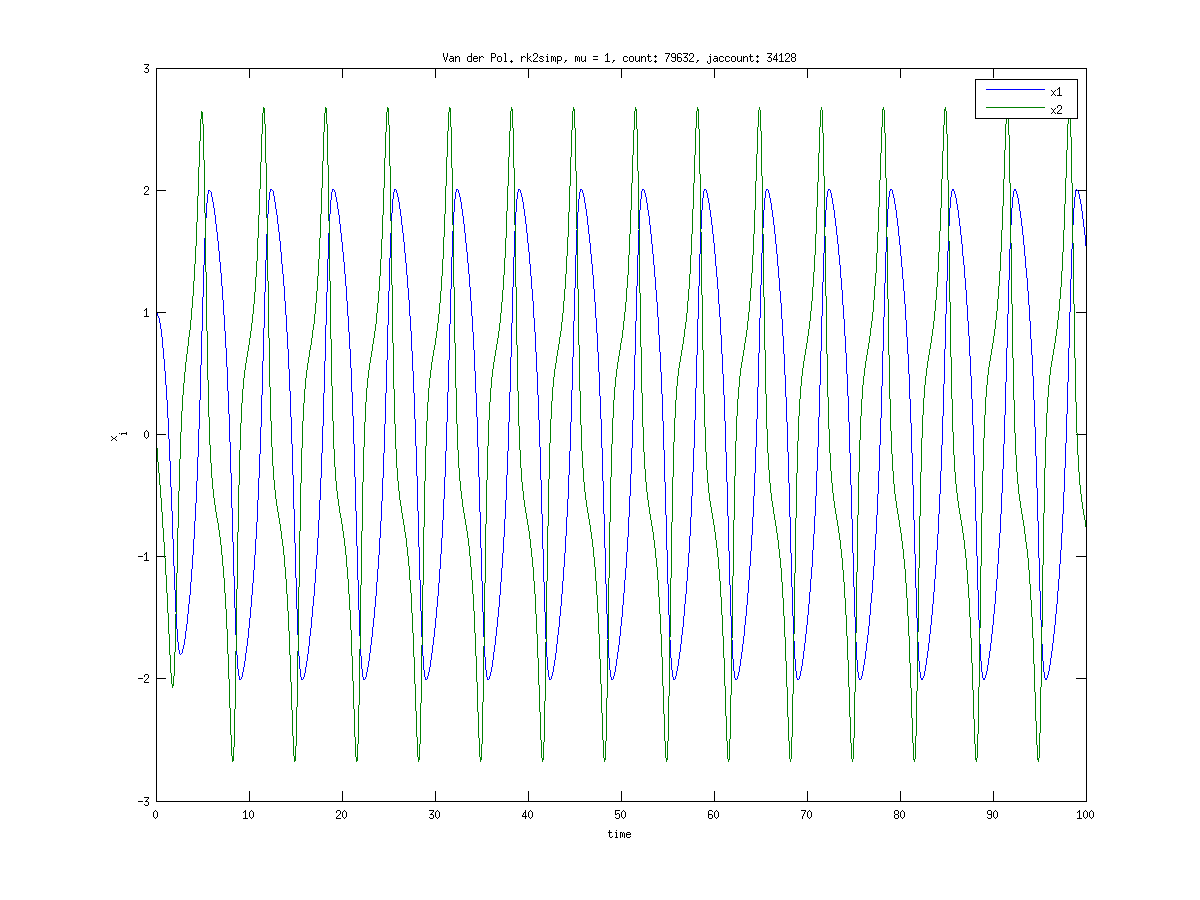
\includegraphics[width=0.8\textwidth]{img/exc1_2_1}
	\caption{Van der Pol model. Solved using rk2simp with parameter $\mu = 1$.}
	\label{fig:exc1_2_1}
\end{figure}

	\FloatBarrier
	\Section{Exercise 2}
	\begin{figure}[h!]
	\centering
	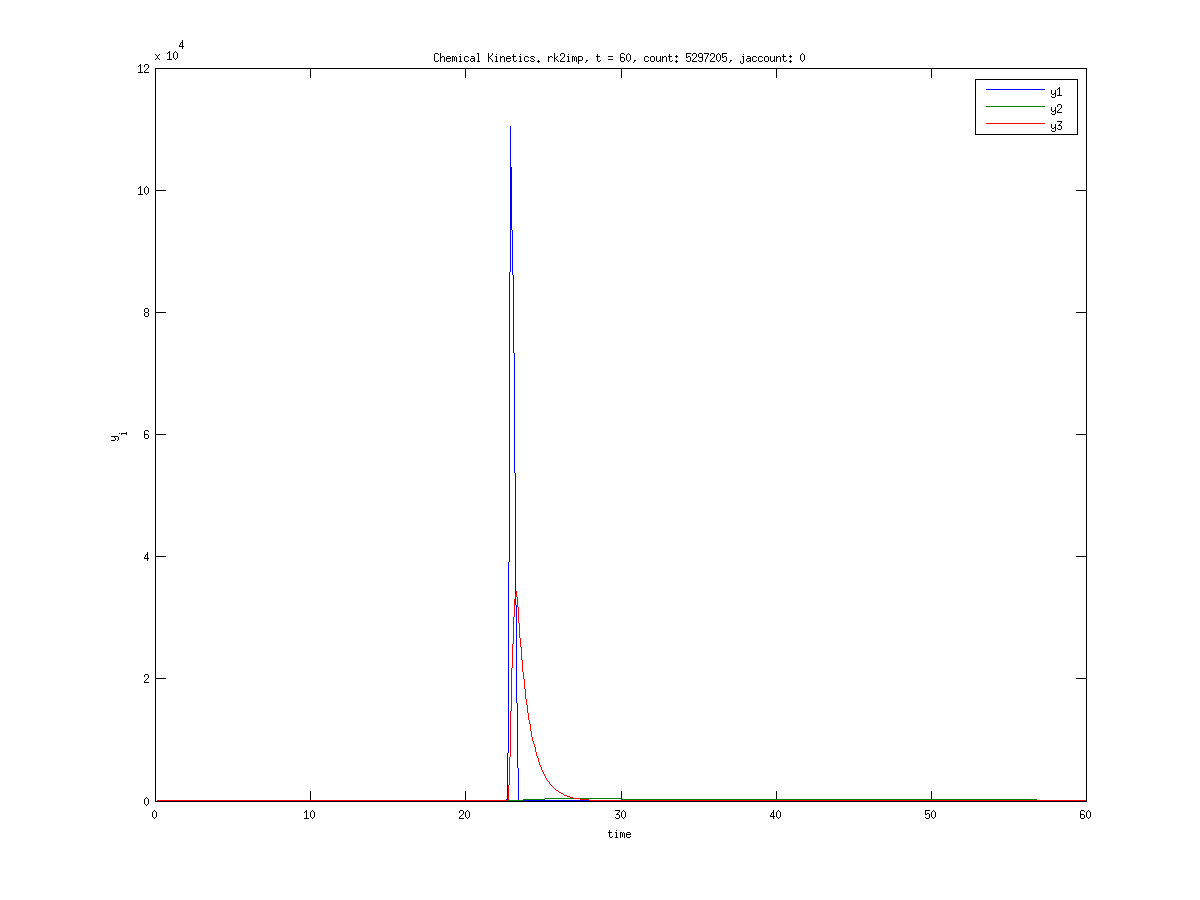
\includegraphics[width=0.8\textwidth]{img/exc2_2_60}
	\caption{Chemical kinetics. Solved using rk2imp integrating from $t=0$ to $t=60$.}
	\label{fig:exc2_2_60}
\end{figure}

\begin{figure}[h!]
	\centering
	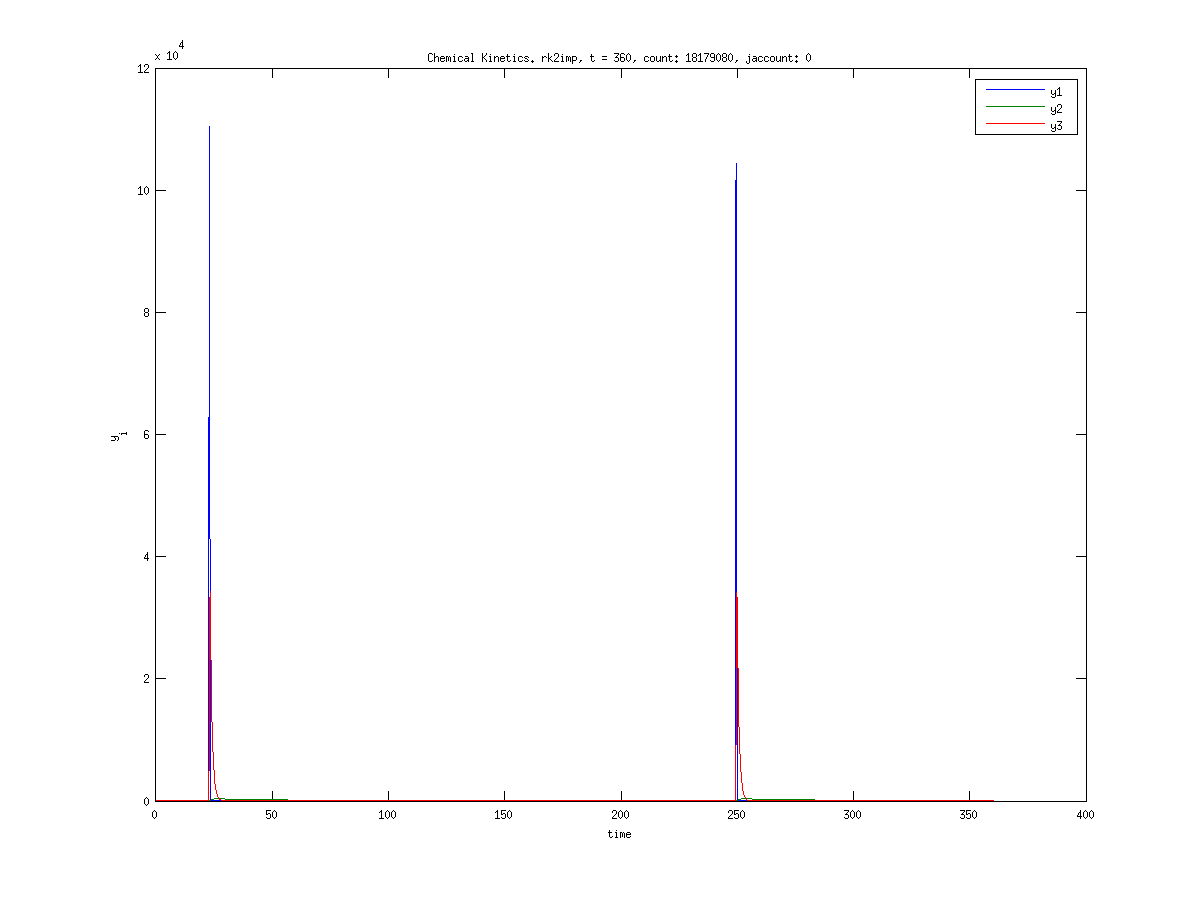
\includegraphics[width=0.8\textwidth]{img/exc2_2_360}
	\caption{Chemical kinetics. Solved using rk2imp integrating from $t=0$ to $t=360$.}
	\label{fig:exc2_2_360}
\end{figure}

\begin{figure}[h!]
	\centering
	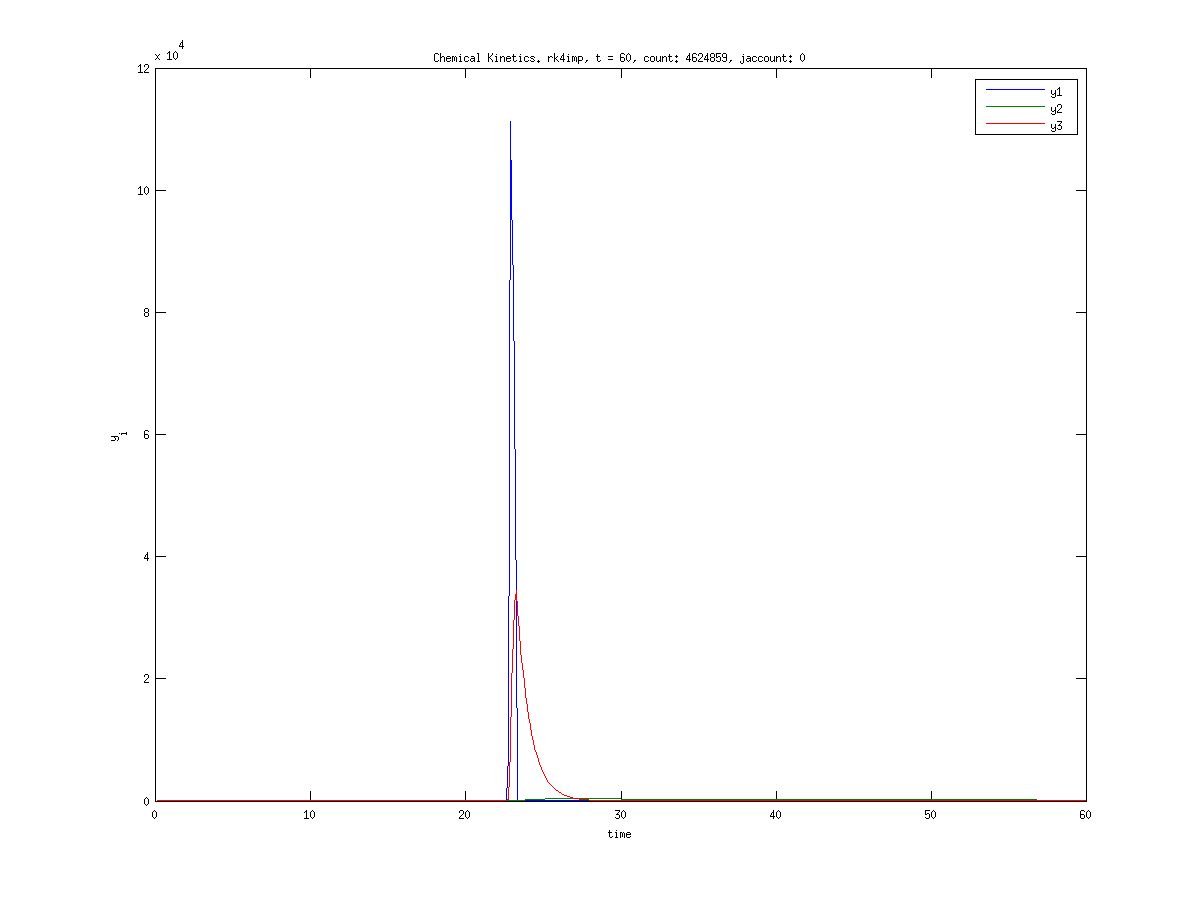
\includegraphics[width=0.8\textwidth]{img/exc2_4_60}
	\caption{Chemical kinetics. Solved using rk4imp integrating from $t=0$ to $t=60$.}
	\label{fig:exc2_4_60}
\end{figure}


\begin{figure}[h!]
	\centering
	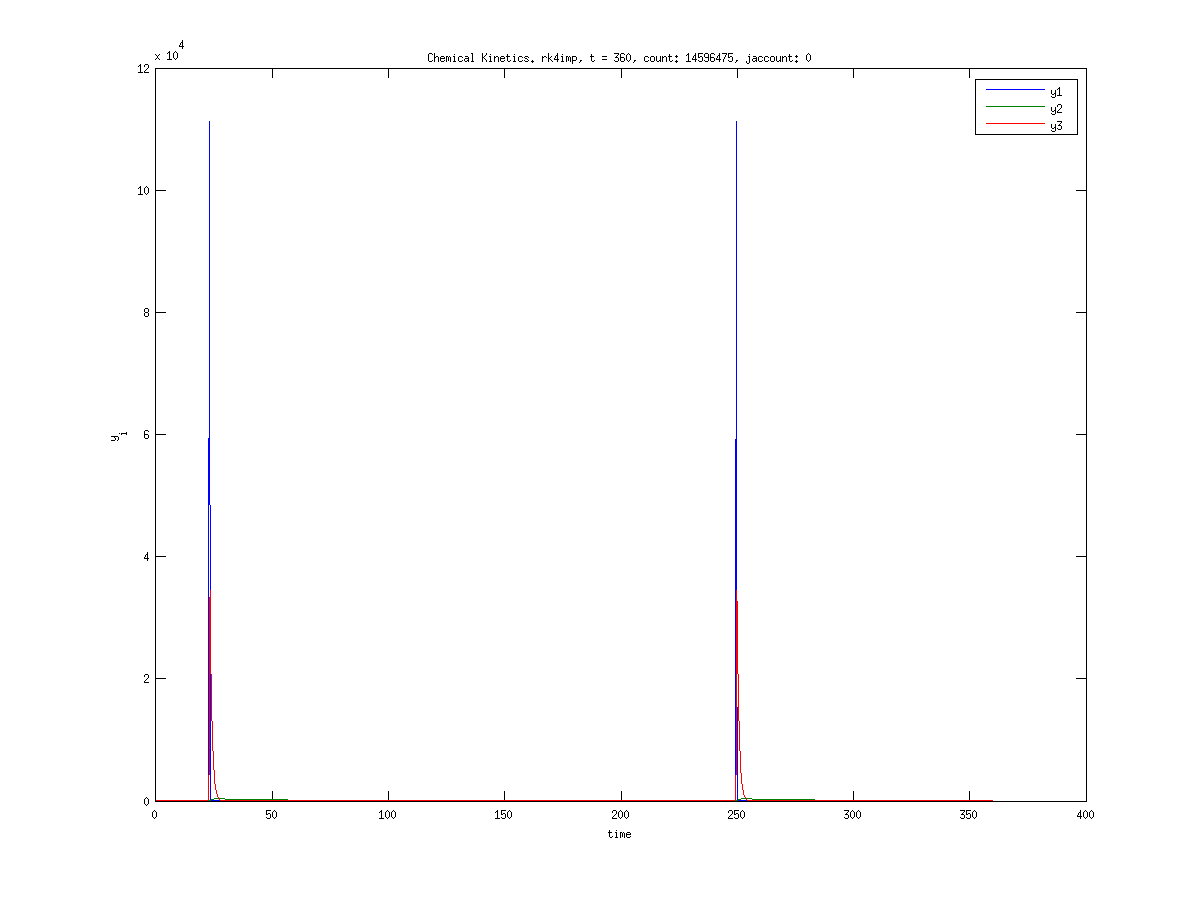
\includegraphics[width=0.8\textwidth]{img/exc2_4_360}
	\caption{Chemical kinetics. Solved using rk4imp integrating from $t=0$ to $t=360$.}
	\label{fig:exc2_4_360}
\end{figure}

The efficiency was about double as fast in the C implementation compared with the matlab implementation. And in the C implementation the rk4imp was better.
The times were: 0.92 seconds from matlab using ode23s; 0.623 seconds in C using rk2imp; 
and 0.419 seconds in C using rk4imp.		

	\FloatBarrier
	\Section{Exercise 3}
	In the previous exercise, the solution for Burger's equation could model the density of cars around a traffic light that turned green on $t=0$.
Another traffic model---but for high-way traffic flow in one lane where a slip road is feeding traffic into the lane---can be modeled using the initial condition
\begin{equation}\label{eq:exc3_pinit}
\rho(x, t=0) = \eta \rho_m e^{-\left(\frac{x-L/4}{L/8}\right)^2}.
\end{equation}
where $0 < \eta \le 1$ is a constant

To investigate the solution of this model. The simulation will be run for 30 time steps (equivalent to 12 seconds); the same parameters values as in exercise 2 are used but with $\eta = 0.1$ as presented in \ref{fig:exc3_congestion_eta01}, here the traffic flows rather smoothly.
If we instead increase $\eta$ to 0.9, adding higher density of traffic as presented in 
\ref{fig:exc3_congestion_eta09} we instead get congestion, increasing the density of traffic at one point at the same time decreasing the velocity at that point.


\begin{figure}[h!]
\begin{subfigure}{.375\textwidth}
	\centering
	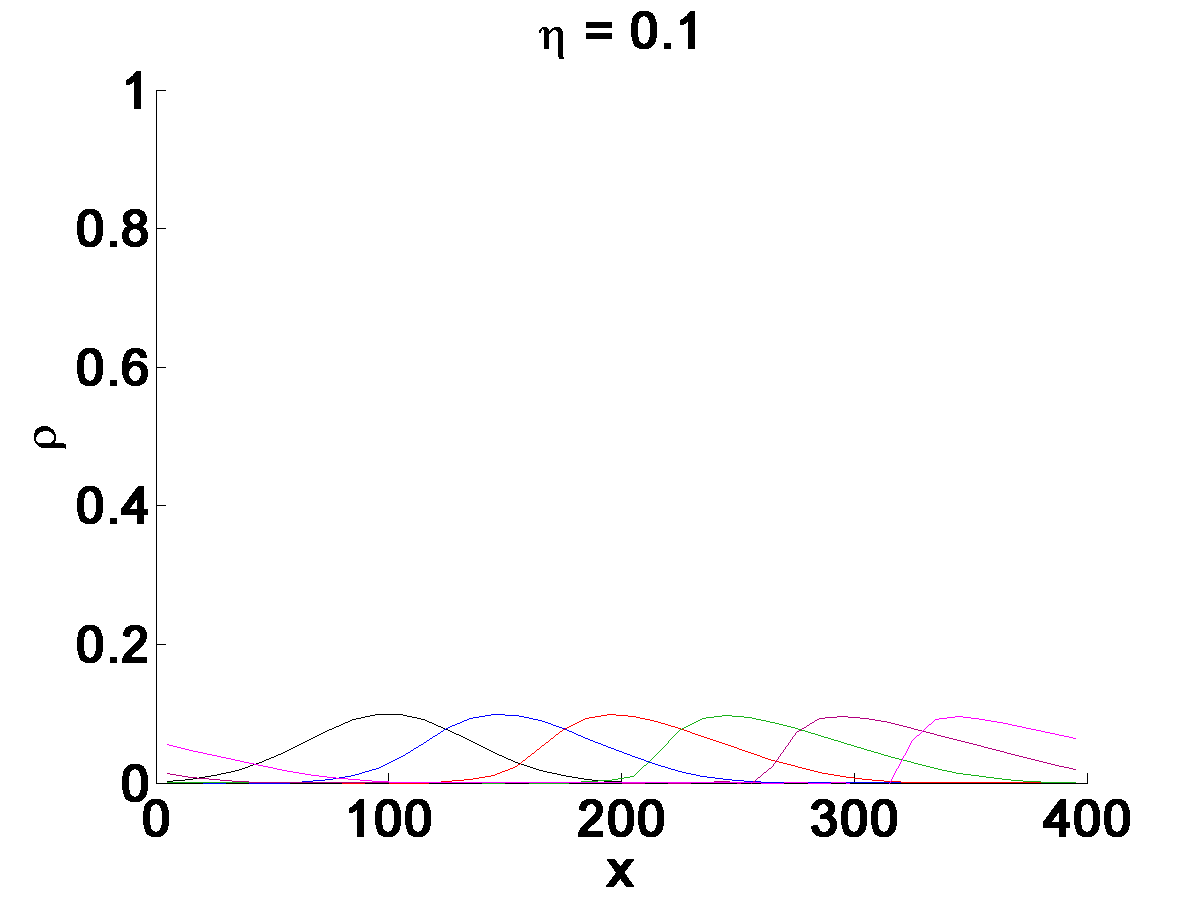
\includegraphics[width=\textwidth]{img/exc3_p_01}
	\caption{}
	\label{fig:exc3_congestion_eta01_p}
\end{subfigure}
\begin{subfigure}{.375\textwidth}
	\centering
	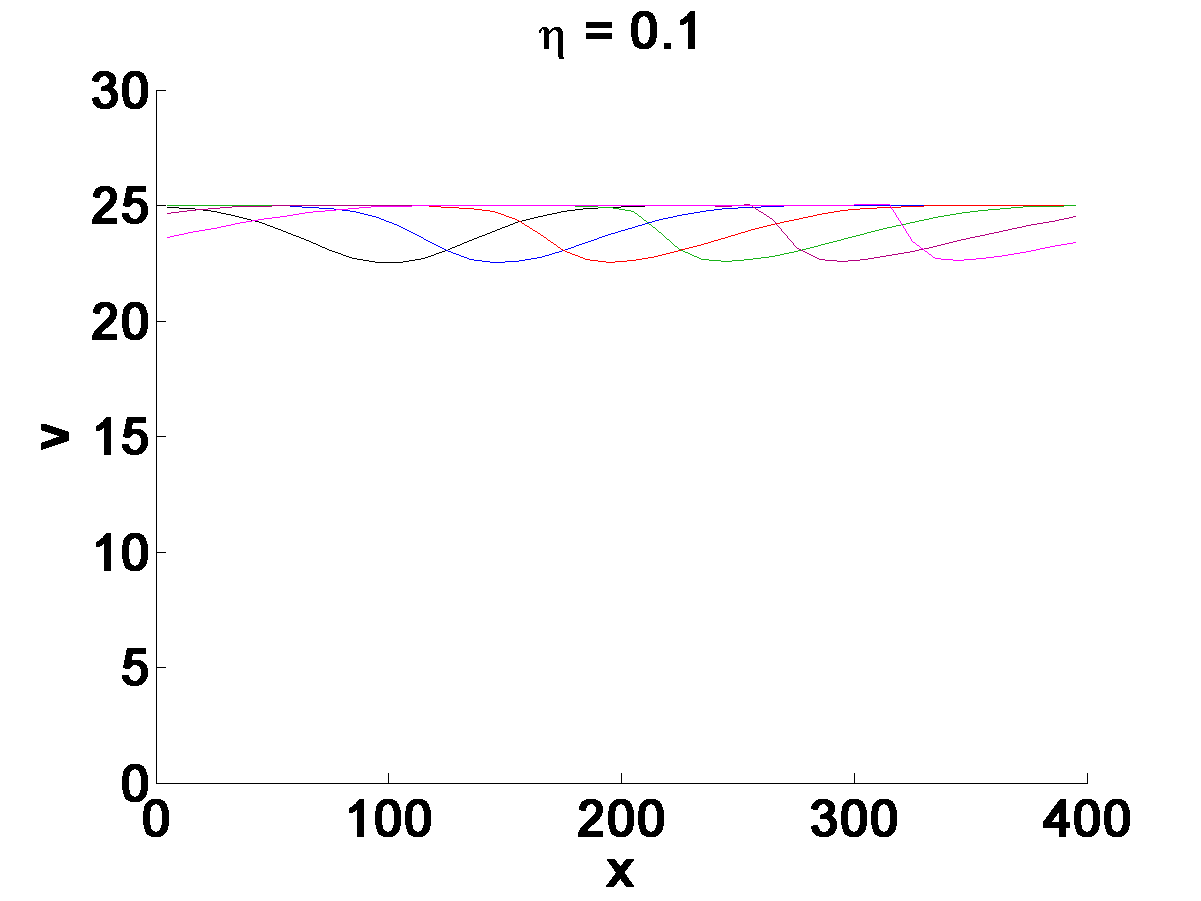
\includegraphics[width=\textwidth]{img/exc3_v_01}
	\caption{}
	\label{fig:exc3_congestion_eta01_v}
\end{subfigure}
\begin{subfigure}{.09\textwidth}
	\centering
	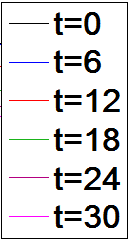
\includegraphics[width=\textwidth]{img/exc3_legend}
\end{subfigure}
\caption{The result of Burger's equation using initial condition $\rho(x, t=0) = \eta \rho_m \exp(-\left((x-L/4)/(L/8)\right)^2)$ with $\eta=0.1$. In (a) is $\rho(x)$ for different times $t$ and in (b) is $v(\rho(x))$ for different times $t$.}
\label{fig:exc3_congestion_eta01}
\end{figure}
\FloatBarrier

\begin{figure}[h!]
\begin{subfigure}{.375\textwidth}
	\centering
	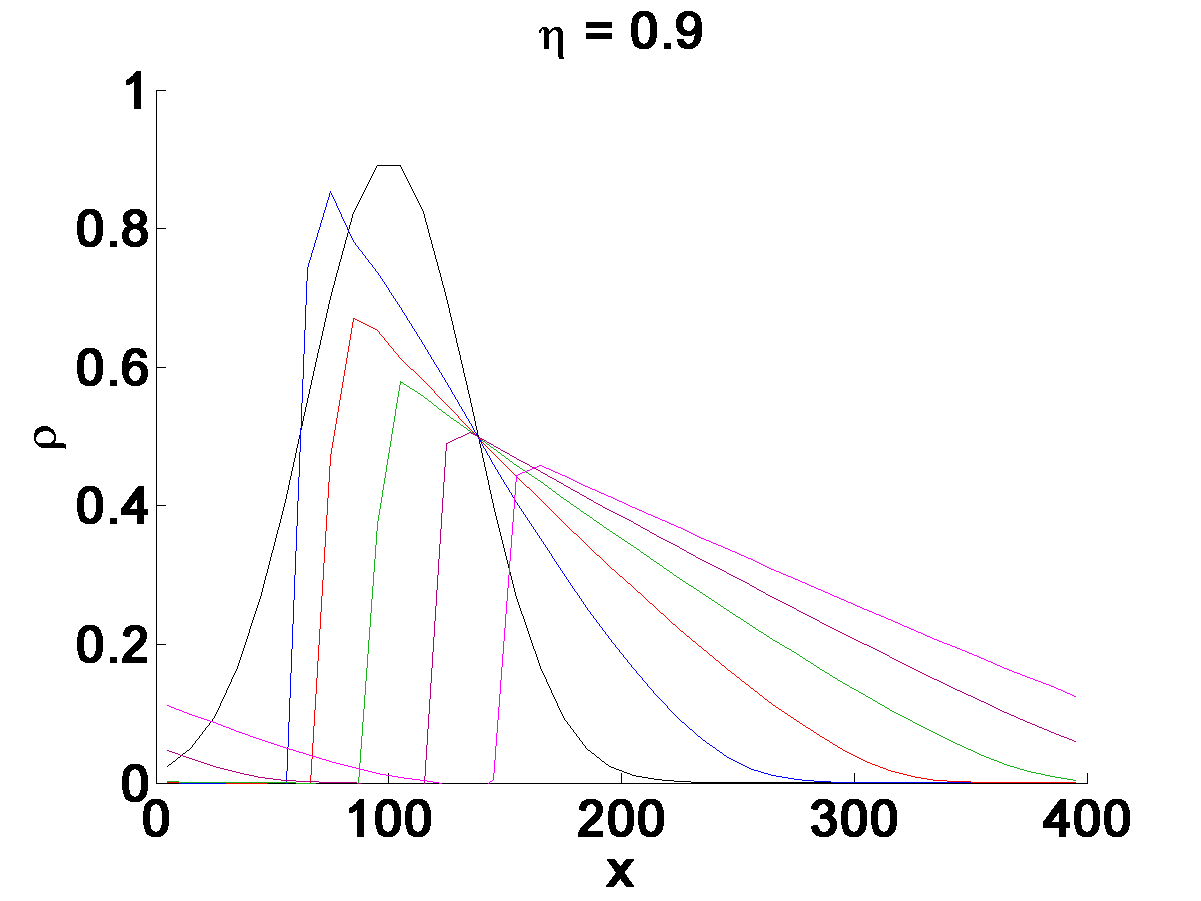
\includegraphics[width=\textwidth]{img/exc3_p_09}
	\caption{}
	\label{fig:exc3_congestion_eta01_p}
\end{subfigure}
\begin{subfigure}{.375\textwidth}
	\centering
	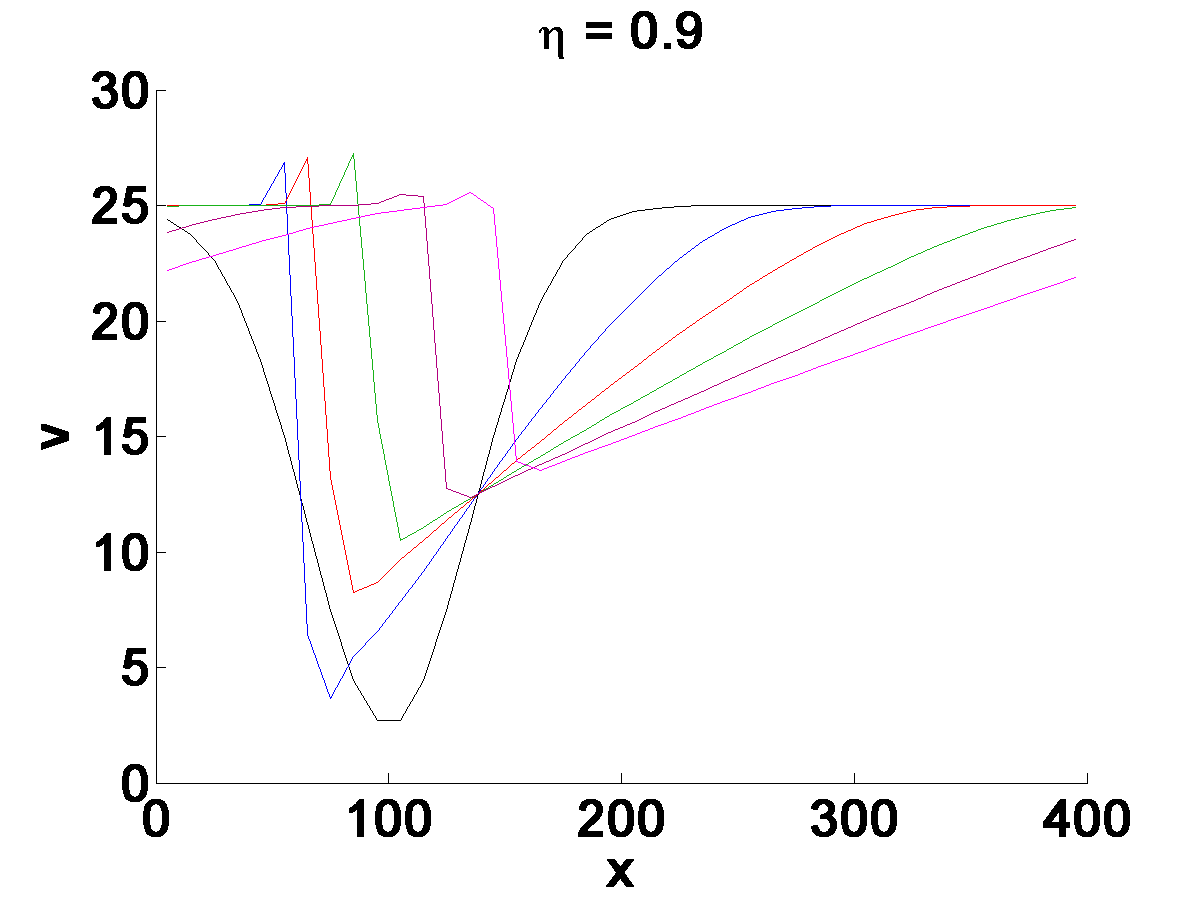
\includegraphics[width=\textwidth]{img/exc3_v_09}
	\caption{}
	\label{fig:exc3_congestion_eta01_v}
\end{subfigure}
\begin{subfigure}{.09\textwidth}
	\centering
	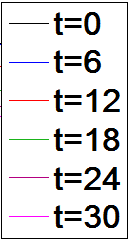
\includegraphics[width=\textwidth]{img/exc3_legend}
\end{subfigure}
\caption{The result of Burger's equation using initial condition $\rho(x, t=0) = \eta \rho_m \exp(-\left((x-L/4)/(L/8)\right)^2)$ with $\eta=0.9$. In (a) is $\rho(x)$ for different times $t$ and in (b) is $v(\rho(x))$ for different times $t$.}
\label{fig:exc3_congestion_eta09}
\end{figure}
\FloatBarrier
	
	\FloatBarrier
	\Section{Exercise 4}
	\begin{figure}[h!]
	\centering
	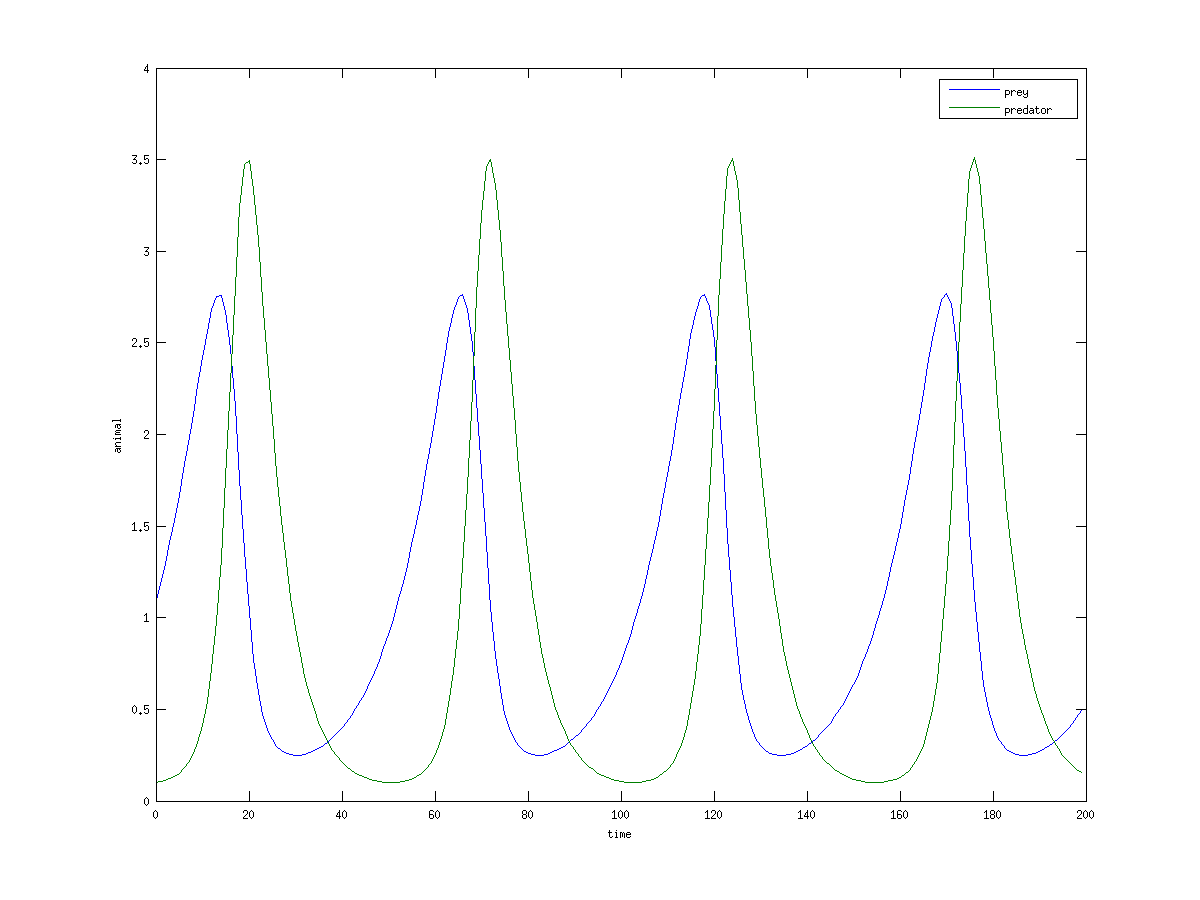
\includegraphics[width=0.8\textwidth]{img/exc4}
	\caption{A predator-prey model. Solved using symplectic Euler A.}
	\label{fig:exc4}
\end{figure}
		

%	% här brjar alla bilagor. Denna måste finnas med även om bara
%	% bilagor anges i \begin{appendices} ... \end{appendices}
%	\appendix
%
%	\Section{Bilaga 1}
%	\ldots{}ligger direkt i dokumentet
%
%	% bilagor, t.ex. källkod. En tom extrasida kommer att skrivas ut för
%	% att få alla sidnummer att stämma
%	\begin{appendices}
%		\appitem{Källkod}{0}
%		\appsubitem{\texttt{mish.c}}{2}
%		\appsubitem{\texttt{mish.h}}{1}
%		\appitem{En bilaga på 3 sidor}{3}
%	\end{appendices}

\end{document}


% Lite information om hur man arbetar med LaTeX
%-----------------------------------------------
%
% LaTeX-koden kan skrivas med en godtycklig editor.
% Fr att "kompilera" dokumentet anvnds kommandot latex:
%    bergner@peppar:~/edu/sysprog/lab1> latex rapportmall.tex
% Resultatet blir ett antal filer, bl.a. en som heter rapportmall.dvi.
% Denna fil kan anvndas fr att titta hur dokumentet egentligen ser
% ut med hjlp av programmet xdvi:
%    bergner@peppar:~/edu/sysprog/lab1> xdvi rapportmall.dvi &
% Du fr d upp ett fnster som visar ditt dokument. Detta fnster
% kommer automatiskt att uppdateras d du ndrar och kompilerar om din
% LaTeX-kod. 
% Nr du anser att din rapport r frdig att skrivas ut anvnder man
% lmpligtvis kommandona dvips och lpr:
%    bergner@peppar:~/edu/sysprog/lab1> dvips -P ma436ps rapportmall.dvi
% Om man vill ha kvar PostScript-filen som dvips genererar kan man gra:
%    bergner@peppar:~/edu/sysprog/lab1> dvips -o rapport.ps rapportmall.dvi
%    bergner@peppar:~/edu/sysprog/lab1> lpr -P ma436ps rapport.ps
% OBS!!! Fr att innehllsfrteckningen och eventuella referenser till
% tabeller och figurer garanterat ska stmma mste man kra latex 2ggr
% p sitt dokument efter att man har ndrat ngot.
%
%
% Lite information om saker man kan tnkas behva i sitt arbete med LaTeX
%-------------------------------------------------------------------------
%
% FORMATTERA TEXT
%
% Fr att formattera text p lite olika stt kan man anvnda fljande LaTeX-
% kommandon:
%    \textbf{denna text kommer att vara i fetstil}
%    \emph{denna text r viktig (kursiv stil)}
%    \texttt{i denna text blir alla tecken lika breda, som med en skrivmaskin}
%    \textsf{denna text visas med ett typsnitt utan serifer}
%
%
% MATEMATISKA FORMLER
%
% Fr att typstta matematiska formler kan man anvnda:
%    $f(x) = x^2 - 3$, vilket lgger in formeln i texten, eller
%    \begin{displaymath}
%        g(x) = \frac{\sin x}{x}
%    \end{displaymath}, vilket lter formeln visas centrerat p en egen rad
% Om du vill att en formel ska numreras byter du ut displaymath mot equation.
% Det finns massor med matematiska symboler, vilket gr att man behver
% ngon liten manual att titta i om man ska konstruera avancerade formler.
% Se slutet p filen fr lite rd om var du kan hitta sdana.
%
%
% INFOGA FIGURER
%
% Fr att infoga en figur kan man gra p fljande stt:
%    \begin{figure}[htb]
%        \includegraphics[scale=0.5, angle=90]{exec_flow.eps}
%        \caption{Detta r bildtexten}
%        \label{EXECFLOW}
%    \end{figure}
% Om man vill referera till denna bild i texten skulle man d skriva enligt:
%    ...i figur \ref{EXECFLOW} kan man se att...
% Ngra sm frklaringar till figurer:
%    [htb] = talar om hur latex ska frska placera bilden (Here, Top, Bottom)
%            Om du anvnder [!h], innebr det Here!!!
%    scale = kan skala om bilden, om den r skalbar
%    angle = kan rotera bilden
%    exec_flow.eps = filnamnet p bilden. Notera att formatet .EPS anvnds
% Fr att skapa figurer anvnds lmpligtvis programmet xfig:
%    bergner@peppar:~/edu/sysprog/lab1> xfig &
% Rita (och spara ofta) tills du r klar. Vlj sedan "Export" och exportera
% din figur till EPS-format.
% Om man vill kan man anvnda endast \includegraphics, men det r inte ofta
% man gr det.
%
%
% INFOGA TABELLER
%
% Om man vill skapa en tabell gr man p fljande stt:
%    \begin{table}[htb]
%        \begin{tabular}{|rlp{10cm}|}
%            \hline
%            13 & $17.26$ & En kommentar som kan strcka sig ver flera rader \\
%            \hline
%        \end{tabular}
%        \caption{Tabelltexten...}
%        \label{TBL:MINTABELL}
%    \end{table}
% Om man vill kan man endast anvnda raderna 2-6, dvs f en tabell utan text
% och nummer. Om man gr p detta vis kommer tabellen alltid att lggas p
% det stlle den skrivs i koden, dvs ungefr samma sak som [!h] -> Here!!!
% Ngra frklaringar:
%    l, r, c = vnsterjustera, hgerjustera eller centrera kolumn
%    p{bredd} = skapa en vnsterjusterad kolumn med en viss bredd
%               kan innehlla flera rader text
%    | = en vertikal linje i tabellen
%    \hline = en horisontell linje i tabellen
%    & = kolumnseparator
%    \\ = radseparator
% Tnk p att tabeller oftast ser bttre ut med ganska f linjer.
%
%
% INFOGA KLLKOD ELLER UTDATA FRN TESTKRNINGAR
%
% Om man vill infoga kllkod eller ngot annat liknande, t.ex. utdata frn
% en testkrning r det bra om LaTeX terger utdatan korrekt, dvs en radbrytning
% betyder en radbrytning och 8 mellanslag p rad betyder 8 mellanslag p rad.
% Fr att stadkomma detta anvnds:
%    \begin{verbatim}
%        allt som skrivs hr terges exakt, med skrivmaskinstypsnitt
%    \end{verbatim}
% Oftast finns det dock bttre verktyg fr att skriva ut kllkod. Exempel p
% sdana r a2ps, enscript och atp.
%
%
% NDRA STORLEK P TEXT
%
% Om du vill ndra storleken p ett stycke, t.ex. p din nyss infogade
% testkrning omger du stycket med \begin{STORLEK} \end{STORLEK}, dr
% STORLEK r ngon av:
%    tiny, scriptsize, footnotesize, small, normalsize, large, Large,
%    LARGE, huge, Huge
% Tnk p att inte mixtra fr mycket med storlekar bara.
%
%
% SKAPA LISTOR AV OLIKA SLAG
%
% Det r ganska vanligt att man vill rada upp saker p ngot stt. Fr att
% skapa punktlistor anvnds:
%    \begin{itemize}
%        \item Detta r frsta punkten
%        \item Detta r andra punkten
%    \end{itemize}
% Om man istllet vill ha en numrerad lista kan man anvnda enumerate istllet
% fr itemize. Listor kan anvndas i flera niver
%
%
% MER INFORMATION OM LaTeX
%
% Lite blandad information om LaTeX, lnkar och annat hittar du p
% http://www.cs.umu.se/~bergner/latex.htm
% En del information om rapportskrivning hittar du p
% http://www.cs.umu.se/~bergner/rapport/
% Det finns massor med information om LaTeX p Internet. Ett litet urval:
% http://www.giss.nasa.gov/latex/
%     r en mycket vlfylld sida om LaTeX
% http://wwwinfo.cern.ch/asdoc/WWW/essential/essential.html
%     r en manual som genererats utifrn ett LaTeX-dokument mha latex2html
% http://tex.loria.fr/english/
%     r ett fylligt arkiv av lnkar till LaTeX-dokument p Internet
%
% Min personliga favorit r dock manualen "The Not So Short Introduction to
% LaTeX2e", som finns i DVI-format p ~bergner/LaTeX/lshort2e.dvi
% Dr str i princip allt man behver veta. Det r bara att anvnda xdvi och
% titta efter det du sker, vilket oftast finns dr.
% Om du, precis som jag, vill kunna leka med mnga kommandon i LaTeX finns en
% "LaTeX Command Summary" p ~bergner/LaTeX/latexcmds.ps
